%% generato automaticamente da tools/build_tex.py --- non modificare
\chapter{Un prodotto che vale $k^{-(k-1)}$}
\label{cap:fattorazionale}
\quaderno{fattorazionale.dfw}{07 Jan 2011}{14}

Gennaio 2011. Quattordici righe, undici delle quali sono valori numerici: il quaderno calcola un prodotto per $k$ da $2$ a $12$ e lascia parlare i risultati. La regolarità si vede a occhio nudo, e la dimostrazione — che il quaderno non scrive — sta in due passaggi.

\section{Il prodotto e i suoi valori}

L'oggetto studiato è il prodotto delle differenze fra i reciproci dei primi $k-1$ interi e il reciproco di $k$.

\begin{espr}{1}{User}{}
\[
\prod_{n=1}^{k - 1} \left(\frac{1}{n} - \frac{1}{k}\right)
\]
\end{espr}
Il prodotto studiato: $k-1$ fattori, tutti della forma $1/n-1/k$.

\begin{espr}{2}{Simp(Sub(\#1))}{}
\[
\frac{1}{2}
\]
\end{espr}
$k=2$: un solo fattore, $1-1/2$.

\begin{espr}{3}{Simp(Sub(\#1))}{}
\[
\frac{1}{9}
\]
\end{espr}
$k=3$: il valore è $1/9=1/3^2$.

\begin{espr}{4}{Simp(Sub(\#1))}{}
\[
\frac{1}{64}
\]
\end{espr}
$k=4$: $1/64=1/4^3$.

\begin{espr}{5}{Simp(Sub(\#1))}{}
\[
\frac{1}{625}
\]
\end{espr}
$k=5$: $1/625=1/5^4$.

\begin{espr}{6}{Simp(Sub(\#1))}{}
\[
\frac{1}{7776}
\]
\end{espr}
$k=6$: $1/7776=1/6^5$.

\begin{espr}{7}{Simp(Sub(\#1))}{}
\[
\frac{1}{117649}
\]
\end{espr}
$k=7$: $1/117649=1/7^6$.

\begin{espr}{8}{Simp(Sub(\#1))}{}
\[
\frac{1}{2097152}
\]
\end{espr}
$k=8$: $1/2\,097\,152=1/8^7$.

\begin{espr}{9}{Simp(Sub(\#1))}{}
\[
\frac{1}{43046721}
\]
\end{espr}
$k=9$: $1/43\,046\,721=1/9^8$.

\begin{espr}{10}{Simp(Sub(\#1))}{}
\[
\frac{1}{1000000000}
\]
\end{espr}
$k=10$: esattamente un miliardesimo, cioè $1/10^9$. È la riga che rende la regola indiscutibile.

\begin{espr}{11}{Simp(Sub(\#1))}{}
\[
\frac{1}{25937424601}
\]
\end{espr}
$k=11$: $1/11^{10}$.

\begin{espr}{12}{Simp(Sub(\#1))}{}
\[
\frac{1}{743008370688}
\]
\end{espr}
$k=12$: $1/12^{11}$. Undici casi consecutivi, tutti conformi.

\begin{figure}[htbp]
  \centering
  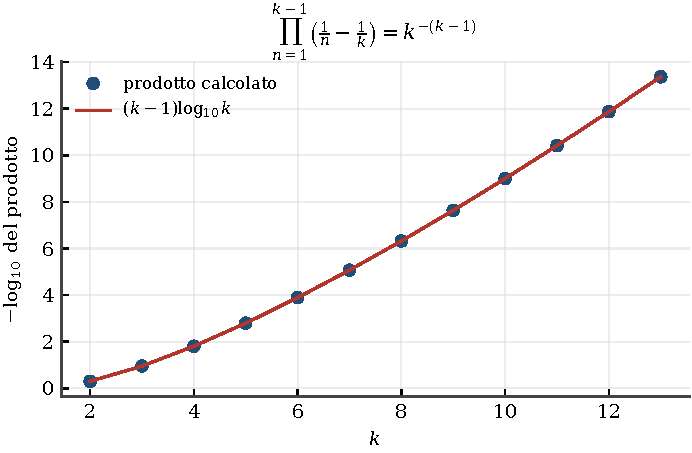
\includegraphics[width=0.86\linewidth]{../figures/fattorazionale.pdf}
  \caption{I dodici valori calcolati nel quaderno, in scala logaritmica, confrontati con la retta $(k-1)\log_{10}k$. La coincidenza è esatta, non approssimata.}
  \label{fig:fattorazionale}
\end{figure}

I valori sono $\tfrac12,\ \tfrac19,\ \tfrac1{64},\ \tfrac1{625},\ \tfrac1{7776},\ \tfrac1{117649},\dots$ e i denominatori sono $2^1,\ 3^2,\ 4^3,\ 5^4,\ 6^5,\ 7^6$: si tratta di $k^{k-1}$. La riga $\#10$ lo rende evidente anche a chi non stesse guardando: per $k=10$ il prodotto vale esattamente un miliardesimo.

La dimostrazione è breve. Scrivendo ogni fattore come $\dfrac1n-\dfrac1k=\dfrac{k-n}{nk}$, il prodotto diventa
\[
  \prod_{n=1}^{k-1}\frac{k-n}{nk}
  =\frac{\displaystyle\prod_{n=1}^{k-1}(k-n)}{k^{\,k-1}\displaystyle\prod_{n=1}^{k-1}n}
  =\frac{(k-1)!}{k^{\,k-1}\,(k-1)!}
  =\frac{1}{k^{\,k-1}},
\]
perché al numeratore compaiono gli stessi fattori del denominatore, soltanto in ordine inverso. Il nome del file — «fattoriale razionale» — allude proprio a questo: due fattoriali che si cancellano lasciando una potenza.

\section{Le due generalizzazioni}

Le ultime due righe provano ad allargare il risultato in due direzioni diverse, entrambe lasciate senza risposta.

\begin{espr}{13}{User}{}
\[
i!\, \prod_{n=1}^{k - 1} \left(\frac{1}{n} - \frac{1}{k}\right)
\]
\end{espr}
Una prima generalizzazione: il prodotto moltiplicato per un fattoriale.

\begin{espr}{14}{User}{}
\[
\prod_{i=1}^{k - n} \left(\frac{1}{i} - \frac{n}{k}\right)
\]
\end{espr}
Una seconda: il reciproco di $k$ viene sostituito da $n/k$ e il numero di fattori scende a $k-n$. Con questa modifica la cancellazione fra numeratore e denominatore non avviene più.


La riga $\#13$ moltiplica il prodotto per un fattoriale, il che equivale a chiedersi che cosa resti di $i!/k^{\,k-1}$. La riga $\#14$ è più interessante: introduce un parametro $n$ nel secondo termine e accorcia di conseguenza il numero di fattori. Ripetendo il conto si trova
\[
  \prod_{i=1}^{k-n}\left(\frac1i-\frac nk\right)
  =\frac{1}{k^{\,k-n}}\prod_{i=1}^{k-n}\frac{k-ni}{i},
\]
e il numeratore non si semplifica più con $i!$ a meno che $n=1$. La regolarità trovata è dunque un caso particolare felice, non l'inizio di una famiglia.

\section*{In sintesi}
\addcontentsline{toc}{section}{In sintesi}

Undici valori numerici e una regola che li spiega tutti. Il quaderno si ferma un attimo prima della dimostrazione, che pure è di due righe — ma i valori scelti, e in particolare quello per $k=10$, sono disposti in modo che la regola si legga da sola.

